\chapter{Appendix I}
\section{Part A}
\begin{table}[h] % Electricity in SA
\centering
\begin{tabular}{| l | r |}\hline
Production from: & Electricity [GWh]:\\\hline
- coal & 239~344 \\
- oil & 194 \\
- gas & 0 \\
- biofuels & 293 \\
- wast & 0 \\
- nuclear & 13~073 \\
- hydro (incl. PSP) & 4~860 \\
- geothermal & 0 \\
- solar PV & 50 \\
- solar thermal & 0 \\
- wind & 103 \\
- tide & 0 \\
- other sources & 0 \\\hline
Total production: & 257~919 \\\hline
Imports & 10 006 \\
Exports & -15~035 \\\hline
Domestic supply: & 252~890 \\\hline
Statistical differences & -2 769 \\
Energy industry own use & 30~678 \\
Losses & 22~351 \\\hline
Final consumption: & 197~092\\\hline
Industry & 117~272 \\
Transport & 3~826 \\
Residential & 38~779\\
Commercial and public services & 28~183 \\
Agriculture / forestry  & 5~709 \\
Other non-specified & 3~323 \\\hline
\end{tabular}
\caption[Electricity flow in South Africa 2012.]{Electricity flow in South Africa 2012\cite{Agency2015}.}\label{tab1}
\end{table}
\pagebreak
\begin{figure}[h]  
\centering
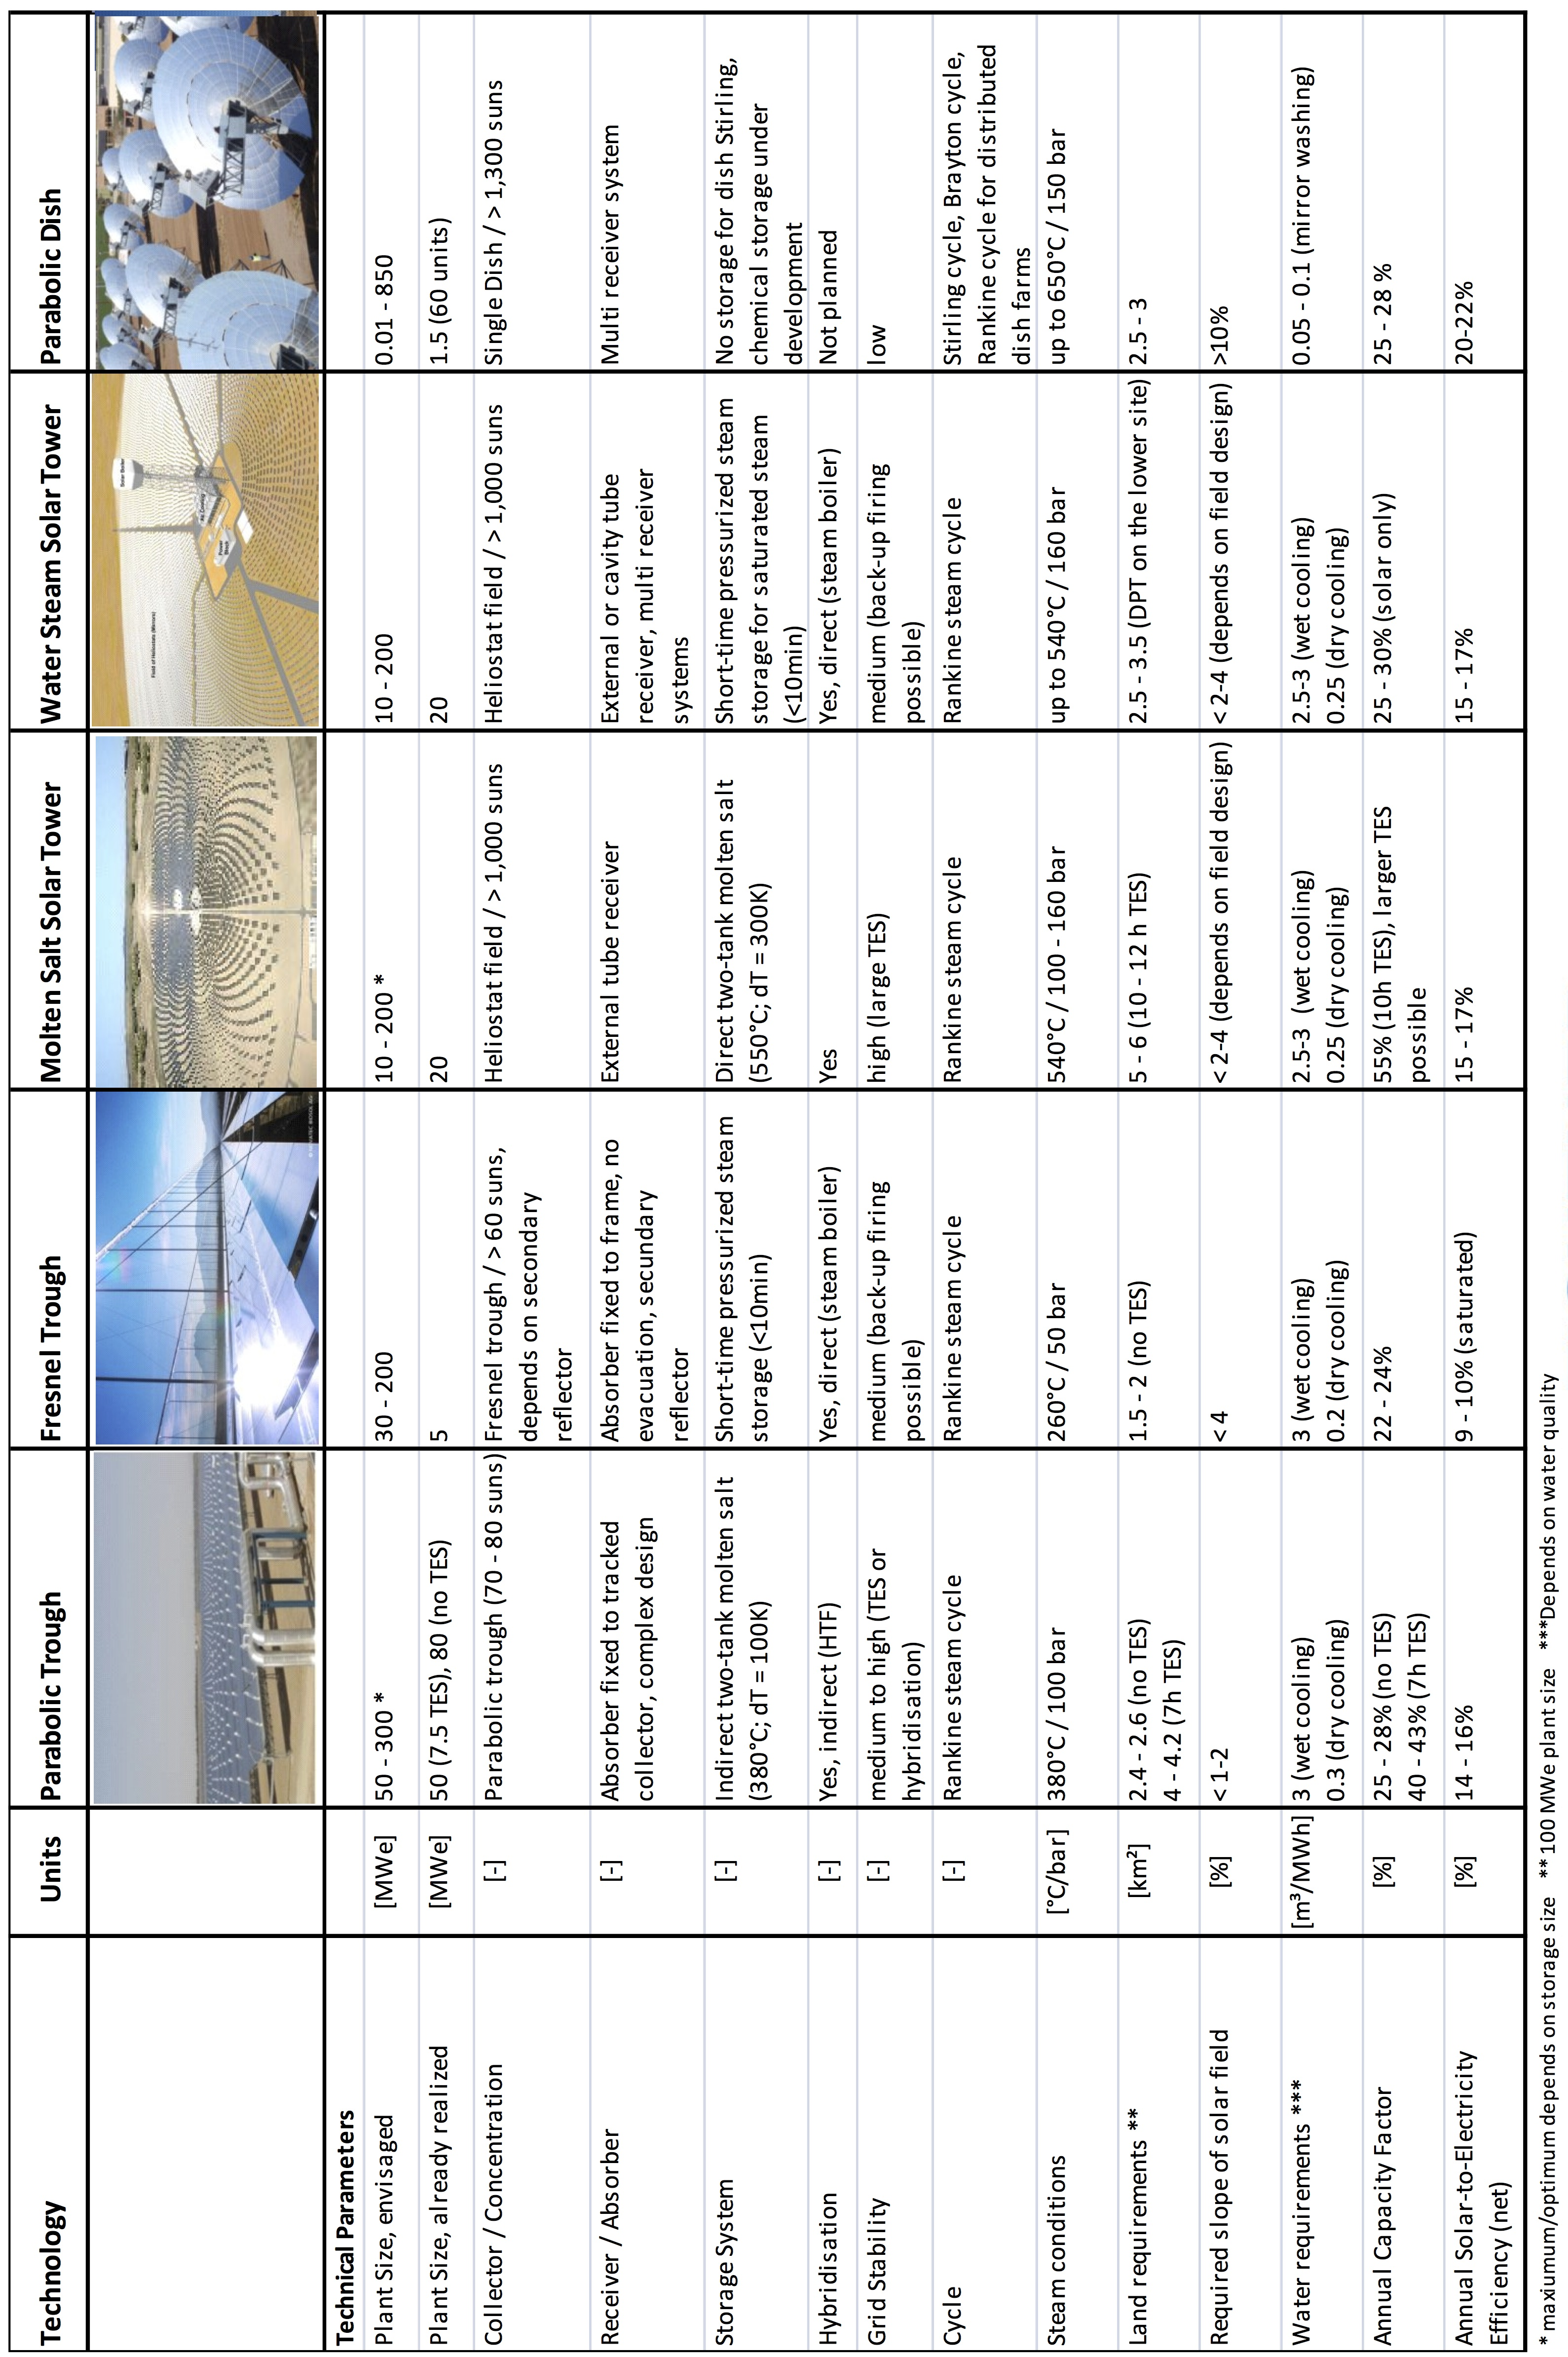
\includegraphics[height=0.95\textheight]{FIG/CSPOverview1}
\caption[CSP Technologies – Comparison I]{CSP Technologies – Comparison I \cite{Fichtner2010}.}\label{CSPOverview1}
\end{figure}
\begin{figure}[h]  
\centering
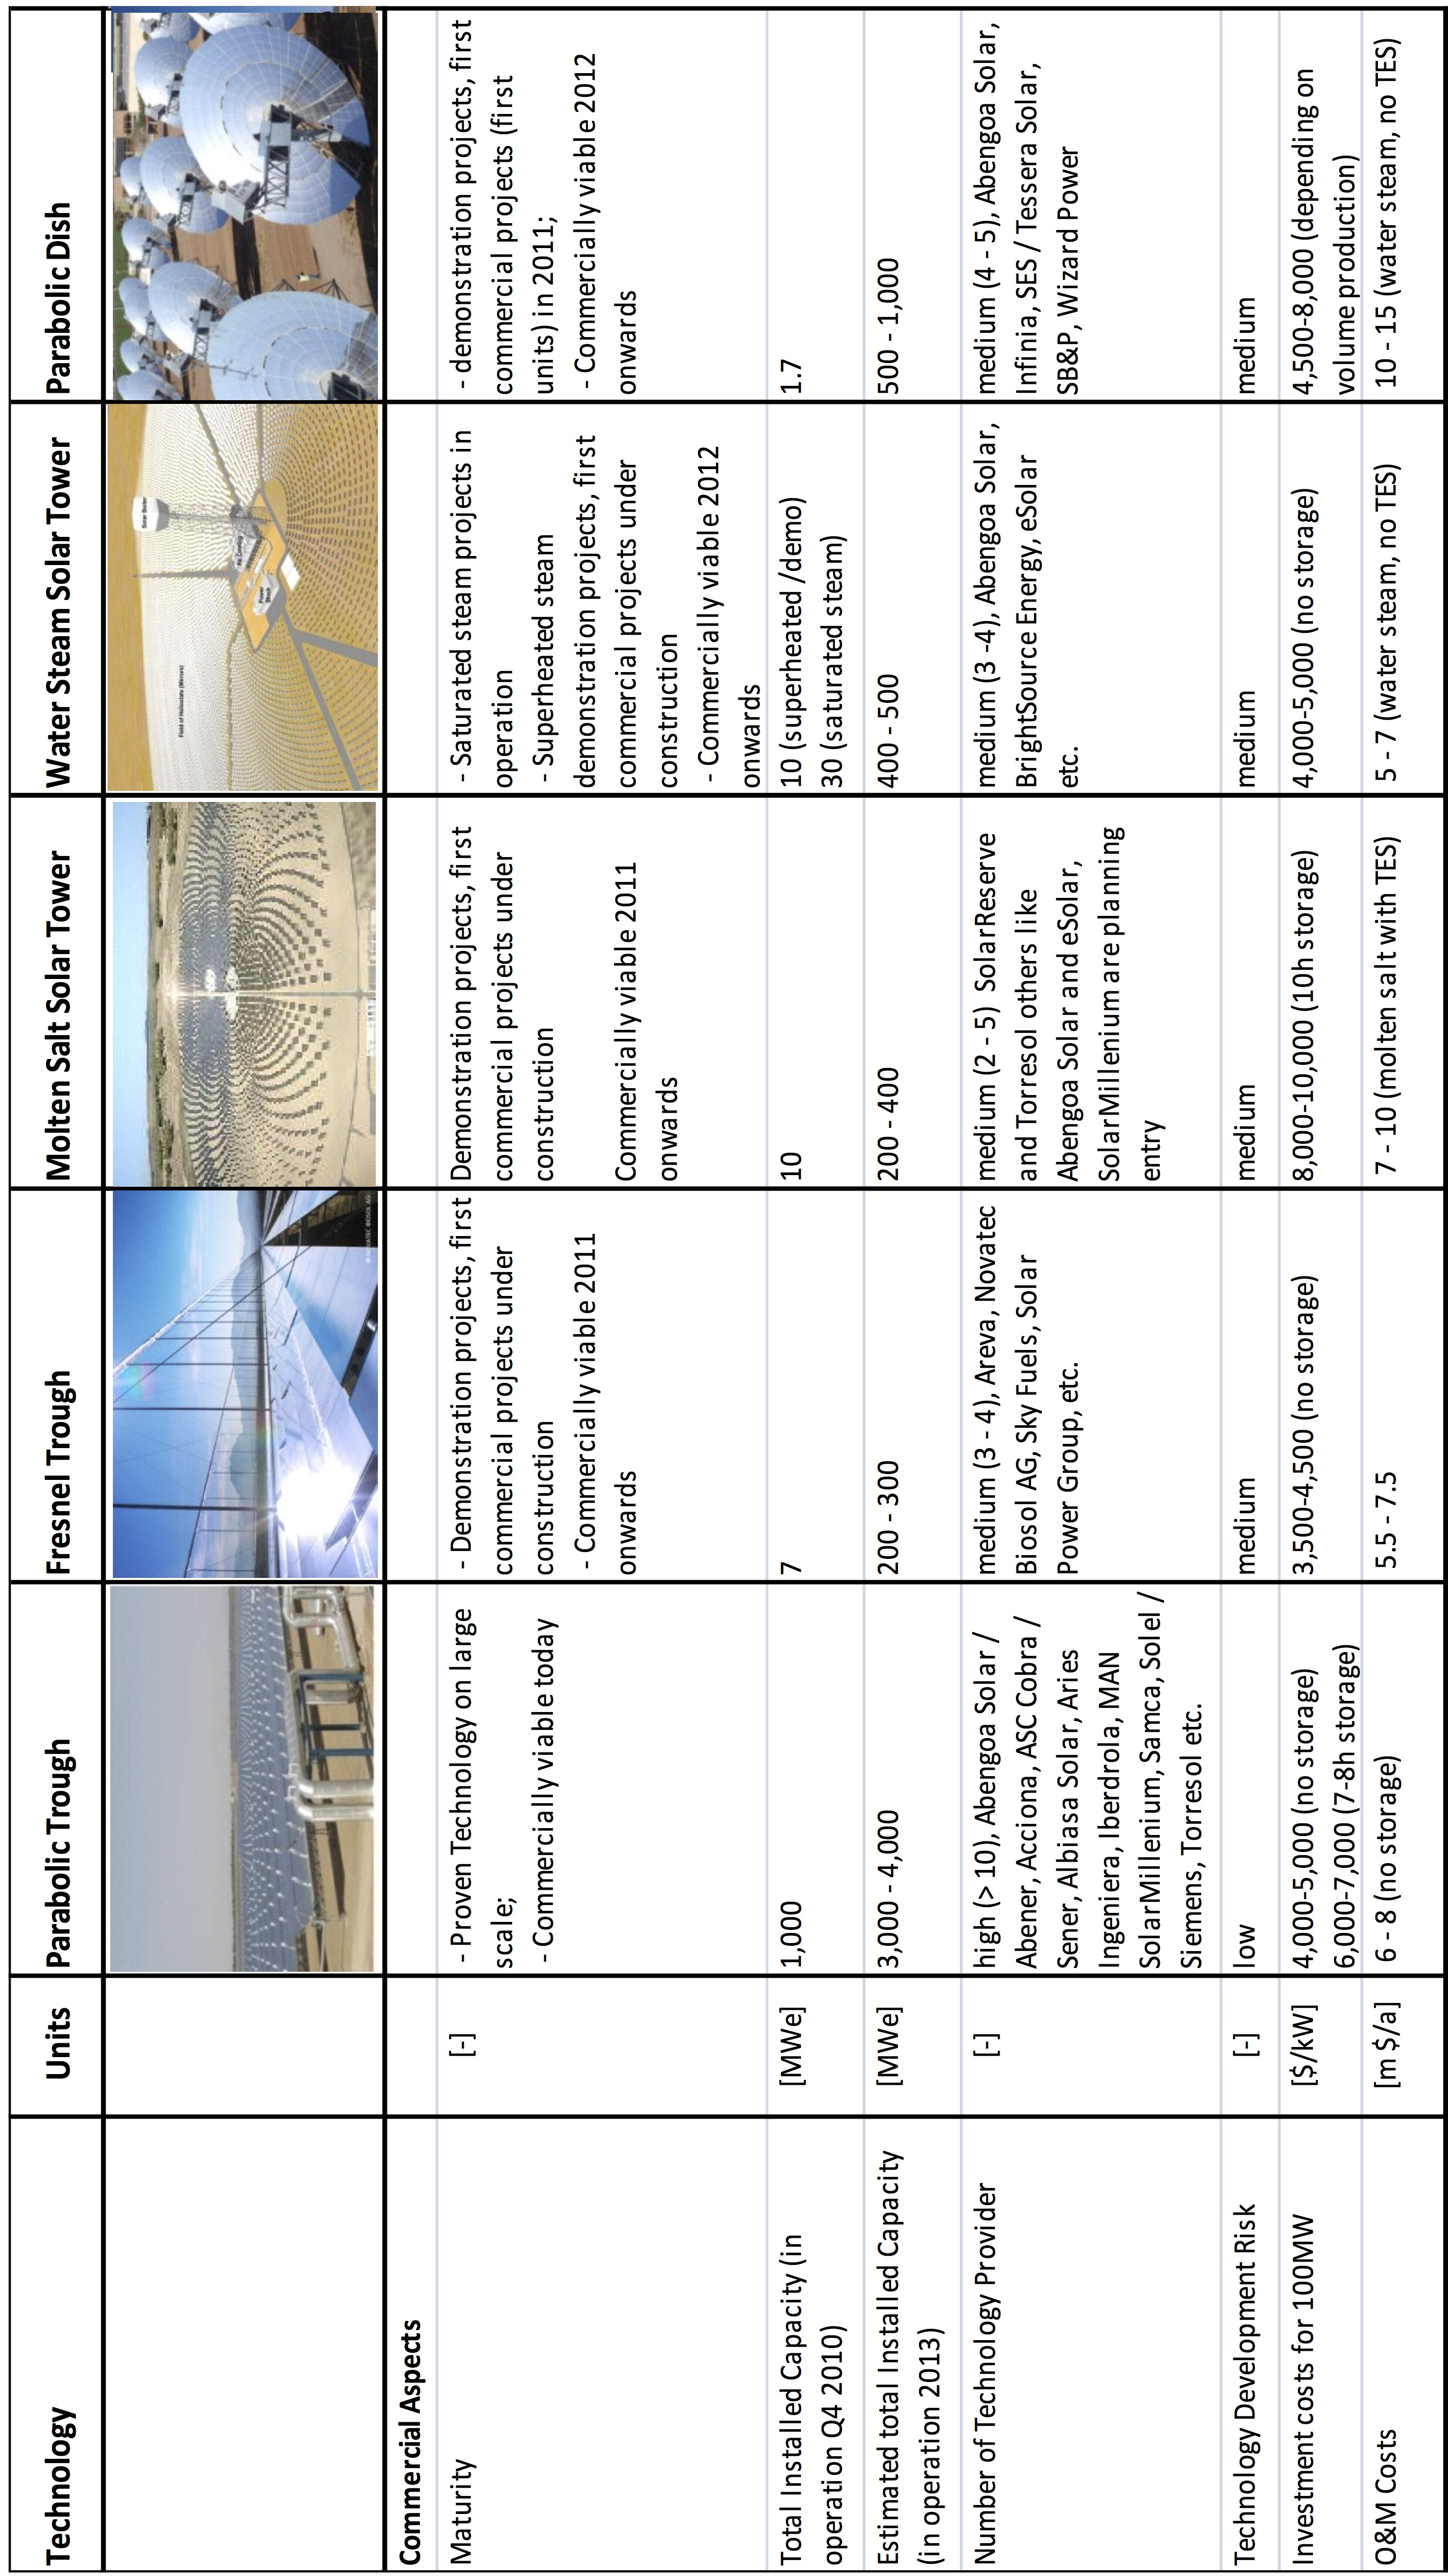
\includegraphics[height=0.95\textheight]{FIG/CSPOverview2}
\caption[CSP Technologies – Comparison I]{CSP Technologies – Comparison II \cite{Fichtner2010}.}\label{CSPOverview2}
\end{figure}
\pagebreak
%
\newpage
